\documentclass[11pt, a4paper, spanish]{article}

%%%%%%%%%% COMIENZO DEL PREAMBULO %%%%%%%%%%

%Info sobre este documento
\author{Martin Cammi}
\title{Trabajo Pr'actico de Ingenier'ia del software I}

%\usepackage{infostyle}                                                  % provee un look & feel similar a un documento Word
\usepackage[top=2.5cm, bottom=2.5cm, left=2.5cm, right=2.5cm]{geometry}  % m\'argenes
\usepackage[ansinew]{inputenc}                                           % permite que los acentos del estilo \'a\'e\'i\'o\'u salgan joya
\usepackage[spanish, activeacute]{babel}                                 % idioma espa\~{n}ol, acentos f\'aciles y deletreo de palabras
\usepackage{indentfirst}                                                 % permite indentar un parrafo a mano
\usepackage{caratula}                                                    % incluye caratula est\'andar
\usepackage{graphicx}                                                    % permite insertar gr\'aficos
\usepackage{color}                                                       % permite el uso de colores en el documento
\usepackage[pdfcreator={TexLive!, LaTeX2e con TeXnicCenter;-)},
			pdfauthor={Grupo 2"},
			pdftitle={Base de Datos - Trabajo practico:},
			pdfsubject={Trabajo Practico de Buffer Manager},
			pdfkeywords={MER, MR},
			pdfstartview=FitH,            % Fits the width of the page to the window
			bookmarksnumbered,            % los bookmarks numerados se ven mejor...
			colorlinks,                   % links con bellos colores
			linkcolor=magenta]            % permite cambiar el color de los links
			{hyperref}                    % Permite jugar con algunas cosas que aparecer\'an en el PDF final
\usepackage{hyperref}
\usepackage{rotating}
\usepackage{ulem}
\usepackage[dash]{dashundergaps}


%\selectlanguage{spanish}

\linespread{1.3}                    % interlineado equivalente al 1.5 l\'ineas de Word...
\pagestyle{myheadings}              %encabezado personalizable con \markboth{}{}
\markboth{}{Trabajo pr\'actico 2 (Cammi, De Sousa) }
\headsep = 30pt                     % separaci\'on entre encabezado y comienzo del p\'arrafo

%\addtolength{\oddsidemargin}{-2cm}	% configuracion IDEAL!!!
%\addtolength{\textwidth}{4cm}
%\addtolength{\textheight}{2cm}

% macro 'todo' para To-Do's
\def\todo#1{\textcolor{red}{#1}}

% Macro 'borde' para un texto con borde
\newsavebox{\fmbox}
\newenvironment{borde}[1]
{\begin{lrbox}{\fmbox}\begin{minipage}{#1}}
{\end{minipage}\end{lrbox}\fbox{\usebox{\fmbox}}\\[10pt]}

%%%%%%%%%% FIN DEL PREAMBULO %%%%%%%%%%

\begin{document}

\materia{Base de Datos}
\submateria{Segundo Cuatrimestre de 2012}
\titulo{Trabajo pr\'actico 2}
\subtitulo{Buffer Manager y estrategias de reemplazo de p'aginas}
\grupo{Grupo 2}

\integrante{Cammi, Mart\'in}{676/02}{martincammi@gmail.com}
\integrante{De Sousa, Mariano}{389/08}{marian\_sabianaa@hotmail.com}

\maketitle

\thispagestyle{empty}

\tableofcontents

\newpage

% Conviene poner las secciones como diferentes archivos,
% sobre todo cuando se trabaja en equipo.
% Es m\'as f\'acil para sincronizar mediante control de versiones.
%\input{Introducci\'on}


% BEGIN Ejemplos de uso

	%\section{Una secci\'on}
	%\label{sec:unaSeccion}
	%Hola! Soy una Secci\'on
	%	\subsection{Una subsecci\'on}
	%		Y yo soy una subsecci\'on!!!
	%		\subsubsection{Una subsubsecci\'on}
	%			Y yo soy una sub-subsecci\'on!!!
	%			\paragraph{Un p\'arrafo\\}
	%				Y yo soy un p\'arrafo, porque no hay mas sub-sub-sub-subsecciones!!!

	%\section{Otra secci\'on}
	%	Como pudimos ver en la secci\'on \ref{sec:unaSeccion}, esto es una demo de una referencia a una secci\'on.
	
	%	Tambi\'en podemos hacer referencia a la p\'agina de la secci\'on:\\[10pt]
	
		% Ejemplo de uso de un borde (falta pulir para que no tire un warning!)
	%	\begin{borde}{0.98\textwidth}
	%		En la p\'agina \pageref{sec:unaSeccion}, hay una secci\'on pilla...
	%	\end{borde}

% END Ejemplos de uso

\newpage 
\section{Investigaci'on sobre estrategia de reemplazo de p'aginas de Oracle}

\subsection{Introducci\'on}

===Hacer referencia bien a la caché indicando que es y el termino caché del buffer de que buffer\\

A lo largo de este trabajo analizaremos el algoritmo de \textit{Touch Count} dise\~{n}ado por \textit{Oracle} para administrar en memoria las p\'aginas que se
traen de la base de datos con el objetivo de evitar los accesos a disco utilizando dicha memoria de a manera m\'as eficiente.\\

Inicialmente Oracle utilizaba para el algoritmo de manejo de \textit{cach\'e} lo que se conoce como algoritmo LRU (Least Recently Used). Este algoritmo, 
descripto m\'as adelante se basa en priorizar en la cach\'e las p\'aginas de disco m\'as referenciadas descartando las menos usadas recientemente 
(definici\'on de LRU).

Un caso muy com\'un que presenta un problema a este algoritmo son los full scan, los cuales recorren todos los registros de una tabla coloc\'andolos en 
la \textit{cach'e} y pisando todo historial previo. As\'i por ejemplo, si la cache del buffer tiene 300 bloques y un escaneo completo de una 
tabla est'a recibiendo 400 bloques en la cache del buffer, todos los bloques populares desaparecer'an. \\

Para superar este problema, Oracle propuso un algoritmo modificado de LRU al que denomin\'o \textit{Touch Count}
  
\subsection{Algoritmo \textit{Touch Count}}

El algoritmo \textit{Touch Count} utiliza el mismo esp\'iritu que sus predecesores LRU y MRU, solo que en una mezcla de ambos. Por un lado priorizar\'a
mantener en la cach\'e las p\'aginas m\'as referenciadas y descartar las menos pero a su modo, cualquier p\'agina que ingrese deber\'a competir 
con otras existentes en la cach\'e por permanecer en la misma, para ello el algoritmo llevar\'a un conteo de cuantas veces fue referenciada. Este n\'umero
de referencias a la p\'agina se denomina \textit{Touch Count}.

\subsection{Problem\'atica que resuelve}

Uno de los problemas que el \textit{Touch Count} resuelve es el de las r\'afagas de acceso a p\'aginas. En un full scan por ejemplo m\'ultiples p\'aginas
son referenciadas y en algoritmos como 

\subsection{Ventajas y desventajas}

\newpage 
\section{Implementaci'on estrategias de reemplazo de p'aginas}

\subsection{Algoritmo de LRU}

El algoritmo LRU (Least Recently Used) funciona de la siguiente manera, intentando mantener en memoria las p\'aginas m\'as recientemente usadas
y en caso de necesitar remover alguna elegir de entre alguna de las menos recientemente usadas.\\

El siguiente es un ejemplo de como las cach\'e se va actualizando mediante el algoritmo LRU.

El siguiente gr\'afico se lee de izquierda a derecha de arriba abajo. La primera hilera de n\'umeros corresponde a la traza de p\'aginas que intentan ser 
accedidas. Debajo de ella aparece en forma vertical la cach\'e y como se va llenando a medida que c\'ada p\'agina de la traza es referenciada.\\ 

Marcaremos con amarillo cuando ocurra un \textit{Hit} y con gris cuando ocurra un \textit{Miss}.
Cuando una p\'agina sea referenciada la marcaremos en la cach\'e en negrita para saber que fue la m\'as recientemente accedida.\\

\begin{center}
		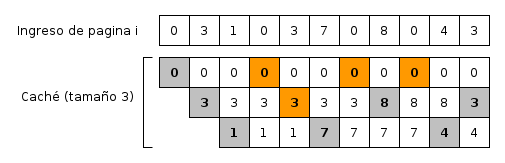
\includegraphics[scale=0.65]{diagramas/LRUAlgorithm.png}\\
\end{center}

As\'i en el ejemplo, 
\begin{itemize}
	\item{ Se referencia inicialmente la p\'agina 0, como la cach\'e se encuentra vac\'ia se produce un \textit{Miss}, y se prodece a agregar
		la p\'agina 0 a la cach\'e.}
	\item{ Se referencia a la p\'agina 3, como no existe en la cach\'e (ya que solo posee la p\'agina 0 agregada anterioremente) se produce 
		un \textit{Miss} y se prodece a agregar la p\'agina 3 a la cach\'e.}
	\item{ Se referencia a la p\'agina 1, como no existe en la cach\'e se produce un \textit{Miss} y se prodece a agregar la p\'agina 1 a la cach\'e.}
	\item{ Se referencia a la p\'agina 0, como existe en la cach\'e se produce un \textit{Hit}. }
	\item{ Se referencia a la p\'agina 3, como existe en la cach\'e se produce un \textit{Hit}. }
	\item{ Se referencia a la p\'agina 7, como no existe en la cach\'e se produce un \textit{Miss} y se prodece a agregar la p\'agina 7 a la cach\'e
		reemplazando la menos recientemente usada que es la p\'agina 1. }
	\item{ Se referencia a la p\'agina 0, como existe en la cach\'e se produce un \textit{Hit}. }
	\item{ Se referencia a la p\'agina 8, como no existe en la cach\'e se produce un \textit{Miss} y se prodece a agregar la p\'agina 8 a la cach\'e
		reemplazando la menos recientemente usada que es la p\'agina 3. }
	\item{ Se referencia a la p\'agina 0, como existe en la cach\'e se produce un \textit{Hit}. }
	\item{ Se referencia a la p\'agina 4, como no existe en la cach\'e se produce un \textit{Miss} y se prodece a agregar la p\'agina 4 a la cach\'e
		reemplazando la menos recientemente usada que es la p\'agina 7. }
	\item{ Se referencia a la p\'agina 3, como no existe en la cach\'e (porque ya fue desalojada) se produce un \textit{Miss} y se prodece a agregar 
		la p\'agina 3 a la cach\'e reemplazando la menos recientemente usada que es la p\'agina 8. }
\end{itemize}

Es interesante notar que una p\'agina no ser\'a desalojada hasta tanto se hayan referenciado al menos una vez a todas las otras, ya que de esta forma
la p\'agina inicial se convertiría en la menos recientemente usada.\\

\noindent{\emph{Cantidad de Hits:} 4} \\
\emph{Cantidad de Miss:} 7, con un total de 3 \emph{Miss} iniciales y 4 \emph{Miss} a lo largo de la traza.\\
\emph{Predicci\'on:} Este enfoque intenta predecir que p\'aginas que fueron referenciadas posiblemente lo sean en un per\'iodo corto de tiempo.\\
\emph{Desventajas:} Una desventaja es que un full scan sobre una tabla barrer\'a por completo con todas las entradas de la cach\'e.\\
\emph{Ventajas:} \\

\newpage
\subsection{Algoritmo de MRU}

El algoritmo MRU (Most Recently Used) funciona a la inversa de \textit{LRU}, intentando mantener en memoria las p\'aginas menos recientemente usadas
y en caso de necesitar remover alguna elegir de entre alguna de las m\'as recientemente usadas.

El siguiente es un ejemplo de como las cach\'e se va actualizando mediante el algoritmo LRU.

\begin{center}
		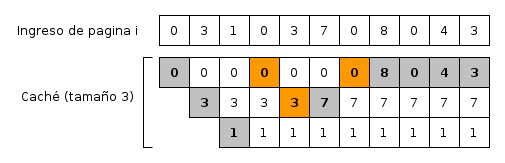
\includegraphics[scale=0.65]{diagramas/MRUAlgorithm.png}\\
\end{center}

El gr\'afico anterior se lee de izquierda a derecha de arriba abajo. La primera hilera de n\'umeros corresponde a la traza de p\'aginas que intentan ser 
accedidas. Debajo de ella aparece en forma vertical la cach\'e y como se va llenando a medida que c\'ada p\'agina de la traza es referenciada.\\ 

Marcaremos con amarillo cuando ocurra un \textit{Hit} y con gris cuando ocurra un \textit{Miss}.
Cuando una p\'agina sea referenciada la marcaremos en la cach\'e en negrita para saber que fue la m\'as recientemente accedida.\\

As\'i en el ejemplo, 

\begin{itemize}
	\item{ Se referencia inicialmente la p\'agina 0, como la cach\'e se encuentra vac\'ia se produce un \textit{Miss}, y se prodece a agregar
		la p\'agina 0 a la cach\'e.}
	\item{ Se referencia a la p\'agina 3, como no existe en la cach\'e (ya que solo posee la p\'agina 0 agregada anterioremente) se produce 
		un \textit{Miss} y se prodece a agregar la p\'agina 3 a la cach\'e.}
	\item{ Se referencia a la p\'agina 1, como no existe en la cach\'e se produce un \textit{Miss} y se prodece a agregar la p\'agina 1 a la cach\'e.}
	\item{ Se referencia a la p\'agina 0, como existe en la cach\'e se produce un \textit{Hit}. }
	\item{ Se referencia a la p\'agina 3, como existe en la cach\'e se produce un \textit{Hit}. }
	\item{ Se referencia a la p\'agina 7, como no existe en la cach\'e se produce un \textit{Miss} y se prodece a agregar la p\'agina 7 a la cach\'e
		reemplazando la m\'as recientemente usada que es la p\'agina 3. }
	\item{ Se referencia a la p\'agina 0, como existe en la cach\'e se produce un \textit{Hit}. }
	\item{ Se referencia a la p\'agina 8, como no existe en la cach\'e se produce un \textit{Miss} y se prodece a agregar la p\'agina 8 a la cach\'e
		reemplazando la m\'as recientemente usada que es la p\'agina 0. }
	\item{ Se referencia a la p\'agina 0, como no existe en la cach\'e (porque ya fue desalojada) se produce un \textit{Miss} y se prodece a agregar 
		la p\'agina 0 a la cach\'e reemplazando la m\'as recientemente usada que es la p\'agina 8. }
	\item{ Se referencia a la p\'agina 4, como no existe en la cach\'e se produce un \textit{Miss} y se prodece a agregar 
		la p\'agina 4 a la cach\'e reemplazando la m\'as recientemente usada que es la p\'agina 0. }
	\item{ Se referencia a la p\'agina 3, como no existe en la cach\'e (porque ya fue desalojada) se produce un \textit{Miss} y se prodece a agregar 
		la p\'agina 3 a la cach\'e reemplazando la m\'as recientemente usada que es la p\'agina 4. }
\end{itemize}

En este algoritmo se puede notar que cualquier referencia a una p\'agina existente en la cach\'e la convierte en la potencial primera v\'ictima 
para ser desalojada en caso de un pr\'oximo \textit{Miss}.\\

\noindent{\emph{Cantidad de Hits:} 3}\\
\emph{Cantidad de Miss:} 8, con un total de 3 \textit{Miss} iniciales y 5 \textit{Miss} a lo largo de la traza. \\
\emph{Predicci\'on:} Este tipo de enfoque intenta basarse en que una vez referenciada una p\'agina no volver\'a a serlo al menos en un cierto per\'iodo
de tiempo en el cual si podr\'ian llegar a serlo p\'aginas m\'as antiguas.\\
\emph{Desventajas:} \\
\emph{Ventajas:} \\

\newpage
\subsection{Algoritmo de Touch Count}

Este algoritmo es la mejora del LRU implementada por \textit{Oracle} describiremos un poco de la estructura interna que utiliza el TouchCount.

El algoritmo Touch Count cuenta con tres elementos principales: una lista, un puntero, y un contador de referencias denominado Touch Count. 
La lista se utilizar\'a para manejar las p\'aginas y las prioridades que se le asignar\'an a cada
una esta lista estar\'a dividida en dos \'areas o regiones. La regi\'on de la izquierda de la lista denominada \textit{regi\'on fria} y la regi\'on inmediata
contigua denominada \textit{regi\'on caliente}.\\

Ambas regiones estar\'an separadas por un puntero, al que llamaremos midPointer, que se encargar\'a de marcar dicha divisi\'on. 
En realidad en la implementaci\'on el \textit{midpointer} estar\'a apuntando el primer elemento de la \textit{regi\'on caliente} cuando haya
elementos en dicha regi\'on o al final de la lista en caso contrario.\\

Por otro lado el algoritmo es configurable y cuenta con varios par\'ametros:

\begin{center}
	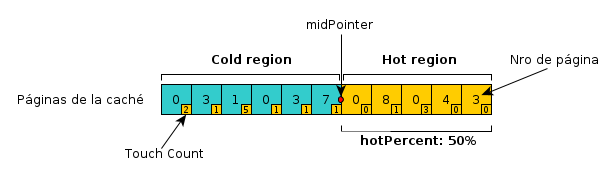
\includegraphics[scale=0.65]{diagramas/TouchCountAlgorithm1.png}\\
\end{center}

\begin{itemize}
	\item{\emph{hotPercent}: Indica el porcentaje de p\'aginas que se quieren mantener en la \textit{regi\'on caliente}. Si el porcentaje no
da exacto se toma la cantidad de p\'aginas que conformen el porcentaje inmediato inferior. }
	\item{\emph{agingTouchTime}: Es la cantidad m\'inima de tiempo a esperar antes de aumentar el Touch Count de una p\'agina ante otra referencia}
	\item{\emph{agingToHotCriteria}: Es el valor al cual se establece al Touch Count de una p\'agina cuando \'esta pasa a la \textit{regi\'on caliente} }
	\item{\emph{agingWhenMoveToHot}: Es el valor minimo de Touch Count que debe tener una p\'agina para que pueda ser enviada a la \textit{regi\'on caliente}}
\end{itemize}

Ahora describiremos su comportamiento en base a las operaciones que se realizan sobre la cach\'e.

\begin{center}
	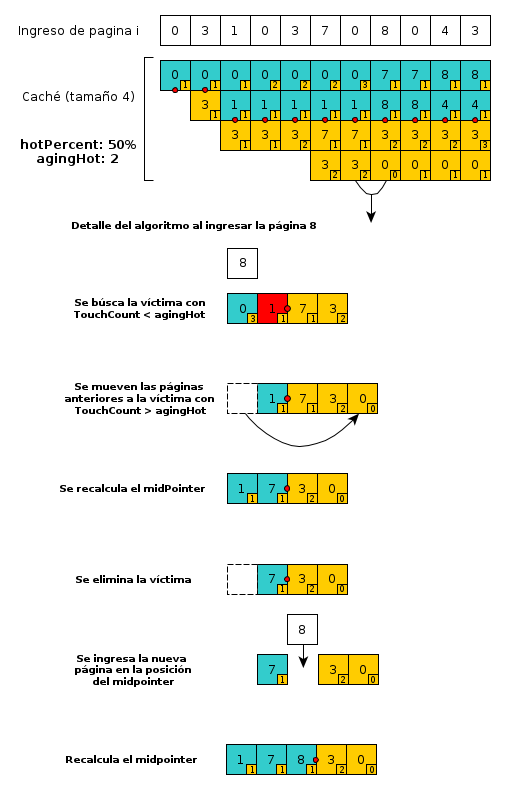
\includegraphics[scale=0.65]{diagramas/TouchCountAlgorithm2.png}\\
\end{center}

Como puede verse en el ejemplo anterior, las operaciones de \textit{agregar}, \textit{encontrar víctima} y \textit{remover} hacen algunas extras que lo que indican a simple vista.

\begin{itemize}
	\item{Agregar una p\'agina:
		Si la cach\'e todav\'ia posee espacio disponible agregar\'a la nueva p\'agina en la posici\'on que indique el \textit{midPointer}.
		Si la cach\'e no posee espacio disponible proceder\'a a buscar una v\'ictima para removerla y agregar la nueva en la posici\'on del \textit{midPointer}.
	}
	\item{Encontrar v\'ictima: }
		El algoritmo comienza buscando una v\'ictima que ser\'a la primera de la regi\'on fria que tenga touch count menor al \textit{agingToHotCriteria}
		Una vez encontrada la v\'ictima, mover\'a todas las p\'aginas que al recorrer hayan superado el  \textit{agingToHotCriteria} al
		final de la \textit{regi\'on caliente} asign\'andole un touch count de 0. Al mismo tiempo por movimiento de estos otra p\'agina pasar\'a
		el umbral de la caliente a la fria como ocurre con la p\'agina 7 del ejemplo anterior al moverse la p\'agina 0 de la \textit{regi\'on fria}
		a la \textit{regi\'on caliente}. A estas p\'aginas que pasan a la \textit{regi\'on fria} se les colocar\'a un touch count de 1.
		
	\item{Remover una p\'agina: }
		El remover una p\'agina borrar\'a la p\'agina de la cach\'e y recalcular\'a la posici\'on del \textit{midpointer}.
\end{itemize}



Peor caso del TouchCount

Si se referencian set de datos diferentes (tablas diferentes) cada vez, no se aclcanzaran para las paginas un aging count suficiente
para salvarlas y todo el tiempo estaremos pisando las p\'agina de la caché con p\'aginas nuevas (al menos en la cola de frias)

Si nada se pasa del agingHot lo que esté en la Hot nunca se va a desaloar, sino que la cola cold ser\'a la que se renueve.
Se le va a dar m\'as importancia a las p\'aginas con touch counte mayor al aging count m\'as nuevas.

\newpage
\section{Test de Unidad}

\subsection{MRUReplacementStrategyTest}

\subsubsection{findVictim tests}

\noindent{\textbf{testNoPageToReplace:} testea que no puede obtenerse una v\'ictima porque todas las p\'aginas est\'an bloqueadas.}\\
\textbf{resultado esperado:} lanzar una PageReplacementStrategyException indicando que \textit{No page can be removed from pool}.\\

\noindent{\textbf{testOnlyOneToReplace:} testea con una \'unica p\'agina no bloqueada.}\\
\textbf{resultado esperado:} devolver la p\'agina no bloqueada como v\'ictima.\\

\noindent{\textbf{testMultiplePagesToReplace: } testea con todas p\'aginas no bloqueadas.}\\
\textbf{resultado esperado:} devolver la primera como v\'ictima.\\

\noindent{\textbf{testMultiplePagesToReplaceButOldestOnePinned: testea con todas p\'aginas no bloqueadas salvo la \'ultima.}}\\
\textbf{resultado esperado:} devolver la primera como v\'ictima.\\

\noindent{\textbf{testMultiplePagesToReplaceWithPinAndUnpin:} testea con todas las p\'aginas no bloqueadas habi\'endoselas hecho pin y unpin a cada una.}  \\
\textbf{resultado esperado:} devolver la primera como v\'ictima.\\

\noindent{\textbf{testMultiplePagesToReplaceWithPinAndUnpinButOneDouble: } testea con todas las p\'aginas no bloqueadas habi\'endoselas hecho pin y unpin,
siendo que la segunda se le hizo un pin unpin m\'as.} \\
\textbf{resultado esperado:} devolver la segunda p\'agina como v\'ictima.\\ 

\noindent{\textbf{testMultiplePagesToReplaceButNewestOnePinnedWithPin: } testea con todas las p\'aginas no bloqueadas habi\'endoselas hecho pin y unpin a cada una
salvo la última a la que s\'olo se le hizo pin al final.}\\
\textbf{resultado esperado:} devolver la segunda p\'agina como v\'ictima. \\

\noindent{\textbf{testMultiplePagesToReplaceButOldestOnePinnedWithPin: } testea con todas las p\'aginas no bloqueadas habi\'endoselas hecho pin y unpin a cada una
salvo la primera a la que s\'olo se le hizo pin al final.}\\
\textbf{resultado esperado:} devolver la segunda p\'agina como v\'ictima. \\


\subsection{LRUReplacementStrategyTest}

\subsubsection{findVictim tests}

\noindent{\textbf{testNoPageToReplace:} testea que no puede obtenerse una v\'ictima porque todas las p\'aginas est\'an bloqueadas.}\\
\textbf{resultado esperado:} lanzar una PageReplacementStrategyException indicando que \textit{No page can be removed from pool}.\\

\noindent{\textbf{testOnlyOneToReplace:} testea con una \'unica p\'agina no bloqueada.}\\
\textbf{resultado esperado:} devolver la p\'agina no bloqueada como v\'ictima.\\

\noindent{\textbf{testMultiplePagesToReplace: } testea con todas p\'aginas no bloqueadas.}\\
\textbf{resultado esperado:} devolver la primera como v\'ictima.\\

\noindent{\textbf{testMultiplePagesToReplaceButOldestOnePinned: testea con todas p\'aginas no bloqueadas salvo la \'ultima.}}\\
\textbf{resultado esperado:} devolver la primera como v\'ictima.\\

\noindent{\textbf{testMultiplePagesToReplaceWithPinAndUnpin:} testea con todas las p\'aginas no bloqueadas habi\'endoselas hecho pin y unpin a cada una.}  \\
\textbf{resultado esperado:} devolver la primera como v\'ictima.\\

\noindent{\textbf{testMultiplePagesToReplaceWithPinAndUnpinFirstReferncedLast: } testea con todas las p\'aginas no bloqueadas habi\'endoselas hecho pin y unpin a cada una
siendo la primera referenciada \'ultima.} \\
\textbf{resultado esperado:} devolver la segunda p\'agina como v\'ictima.\\ 

\noindent{\textbf{testMultiplePagesToReplaceButOldestOnePinnedWithPinAndUnpin: } testea con todas las p\'aginas no bloqueadas habi\'endoselas hecho pin y unpin a cada una
salvo la primera a la que s\'olo se le hizo pin al principio.}\\
\textbf{resultado esperado:} devolver la segunda p\'agina como v\'ictima. \\

\noindent{\textbf{testMultiplePagesToReplaceButOldestOnePinnedWithPinAndUnpinFirstReferencesLast: } testea con todas las p\'aginas no bloqueadas habi\'endoselas hecho pin y unpin a cada una
salvo la primera a la que s\'olo se le hizo pin al final.}\\
\textbf{resultado esperado:} devolver la segunda p\'agina como v\'ictima. \\

\subsection{TouchCountBufferPoolTest}

\subsubsection{TouchCount tests}

\noindent{\textbf{testFindVictimWithSpace:} testea con espacio en la cach\'e.}\\
\textbf{resultado esperado:} lanzar una BufferPoolException indicando que \textit{The buffer still has space}. \\

\noindent{\textbf{testFindVictimWithExistingPage:} testea pasando como par\'ametro una p\'agina a agregar existente en la cach\'e.}\\
\textbf{resultado esperado:} lanzar una BufferPoolException indicando que \textit{The page is already in the buffer}. \\.\\

\noindent{\textbf{testFindVictimInOrder:} testea con todas p\'aginas no bloqueadas.}\\
\textbf{resultado esperado:} devolver la primera como v\'ictima.\\

\noindent{\textbf{testFindVictimAllWithLowTouchCount:} testea con todas p\'aginas con bajo touch count.}\\
\textbf{resultado esperado:} devolver la primera como v\'ictima.\\

\noindent{\textbf{testFindVictimMovingOneToHot:} testea con la primer p\'agina con alto touch count, la segunda con bajo touch count  
y la tercera bloqueada.}\\
\textbf{resultado esperado:} devolver la segunda p\'agina como v\'ictima, además la primera p\'agina debe tener touch count 0 (por haberse movido
a la \textit{regi\'on caliente}), la segunda debe tener touch count 1 (por haberse movido a la \textit{regi\'on fria}) y la tercera no debi\'o
modificar su touch count puesto que no se movi\'o\\

\noindent{\textbf{testFindVictimMovingTwoToHot:} testea con la primer y tercer p\'agina con alto touch count y la segunda con bajo touch count.}\\
\textbf{resultado esperado:} devolver la segunda p\'agina como v\'ictima, además la primera p\'agina debe tener touch count 1 (por haberse movido
a la \textit{regi\'on caliente} primero y a la \textit{regi\'on fria} despu\'es), la segunda debe tener touch count 1 (por haberse movido a la 
\textit{regi\'on fria}) y la tercera touch count 1 por haber terminado en la  \textit{regi\'on fria}.\\

\noindent{\textbf{testMidPointerWithFiftyHotPercentage:} testea el valor del midPointer con hotRegion = 50\%.}\\
\textbf{resultado esperado:} devolver posicion del midPointer en 0 con la cach\'e vac\'ia.\\
\textbf{resultado esperado:} devolver posicion del midPointer en 1 habiendo agregado un elemento.\\
\textbf{resultado esperado:} devolver posicion del midPointer en 1 habiendo agregado dos elementos.\\
\textbf{resultado esperado:} devolver posicion del midPointer en 2 habiendo agregado tres elementos.\\
\textbf{resultado esperado:} devolver posicion del midPointer en 2 habiendo agregado cuatro elementos.\\

\noindent{\textbf{testMidPointerWithThirdHotPercentage:} testea el valor del midPointer con hotRegion = 34\%.}\\
\textbf{resultado esperado:} devolver posicion del midPointer en 0 con la cach\'e vac\'ia.\\
\textbf{resultado esperado:} devolver posicion del midPointer en 1 habiendo agregado un elemento.\\
\textbf{resultado esperado:} devolver posicion del midPointer en 2 habiendo agregado dos elementos.\\
\textbf{resultado esperado:} devolver posicion del midPointer en 2 habiendo agregado tres elementos.\\


\newpage
\section{Trazas evaluadas}

A continuaci\'on hemos confeccionado una serie de trazas para evaluar el comportamiento de cada algoritmo. Algunas trazas intentan identificar
los patrones patol\'ogicos para cada algoritmo analizando cual ser\'ia el escenario de peor caso.

\subsection{ Peor caso MRU: Traza MRUPathological}


	La siguiente traza describe la referencia a p\'aginas que siempre de \textit{Miss}. Para ello se llena la cach\'e (referenciando a las 
p\'aginas 0, 3, 1) que dar\'an \textit{Miss} de inicializaci\'on y luego se referencia una p\'agina que no exista en la cach\'e, la p\'agina 4.
Como la cach\'e est\'a llena, debe desalojar una p\'agina, la 1. Esa ser\'a la p\'agina que se referenciar\'a a continuaci\'on la cual dar\'a \textit{Miss}
y desalojar\'a la p\'agina 4 que fue la \'ultima en ser referenciada y ser\'a la p\'agina que se pedir\'a a continuaci\'on la cual dar\'a \textit{Miss} y
as\'i sucesivamente.

	\begin{center}
	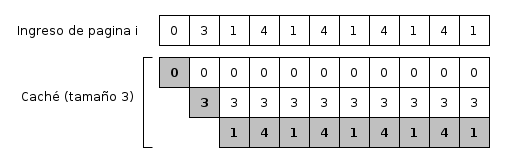
\includegraphics[scale=0.65]{diagramas/MRUPathological.png}\\
	\end{center}


	En la siguiente traza para LRU, se intenta maximizar la cantidad de \textit{Miss} para el algoritmo. El patr\'on para lograrlo se basa
en completar la cach\'e con una traza y luego repetirla varias veces de forma de desalojar las mismas p\'aginas que se mantuvieron al principio.
Al completar la cach\'e se refencia una p\'agina nueva no existente, en el ejemplo la p\'agina 3, se desaloja la p\'agina m\'as antigua, la 0, que 
justamente es la siguiente a ser referenciada por la traza y que vendr\'a a desalojar a la p\'agina 1, que ser\'a justamente la siguiente en ser 
desalojada. De esta forma se ir\'an desalojando las p\'aginas que ser\'an inmediatamente referenciadas ocacionando una serie de \textit{Miss en cascada}. 

de en que se basa
parte de llenar la cach\'e con una traza inicial y luego repetirla nuevamente.  
	
\subsection{ Peor caso LRU}
	\begin{center}
	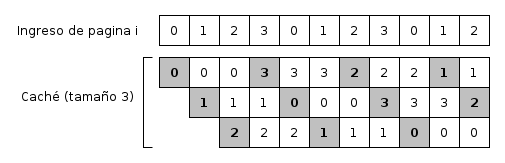
\includegraphics[scale=0.65]{diagramas/LRUPathological.png}\\
	\end{center}

\subsection{ LRU vs TouchCount}

A continuaci\'on se describe un escenario en el cual el algoritmo de Touch Count mejora con respecto a LRU.

El ejemplo consiste en potenciar las p\'aginas que el Touch Count considera importantes, e intentar desalojarlas al mismo tiempo de la cach\'e en el
algoritmo LRU.

Inicialmente se utilizar\'a una traza cualquiera para completar la cach\'e. En ambos algoritmos estar inicializaci\'on dar\'a \textit{Miss} ya que
las p\'aginas no existir\'an.

Un escenario posible ser\'ia

\begin{itemize}
	\item{full scan sobre la tabla A: para cargar las p'aginas en la cach\'e (se asume que los datos de A no superan el tama\~{n}io de la cach\'e}
	\item{varios file scan sobre la tabla A condicionando a los registros con id par: en ambos algoritmos habr\'a \textit{Hit}}
	\item{file scan sobre la tabla A condicionando a los registros con id impar: en ambos algoritmos habr\'a \textit{Hit}}
	\item{file scan sobre la tabla B: en ambos algoritmos habr\'a \textit{Miss}}
	\item{file scan sobre la tabla A: condicionando a los registros con id par: s\'olo en Touch Count las p\'aginas todav\'ia exisit\'ran en cach\'e
ya que las reiteradas referncias del punto 2 habr\'an hecho que Touch Count les diera un pero mayor y por ende las habr\'ia salvado en la \textit{regi\'on caliente}}
\end{itemize}

Conclusion , peso vs ultima accedida.

	\begin{center}
	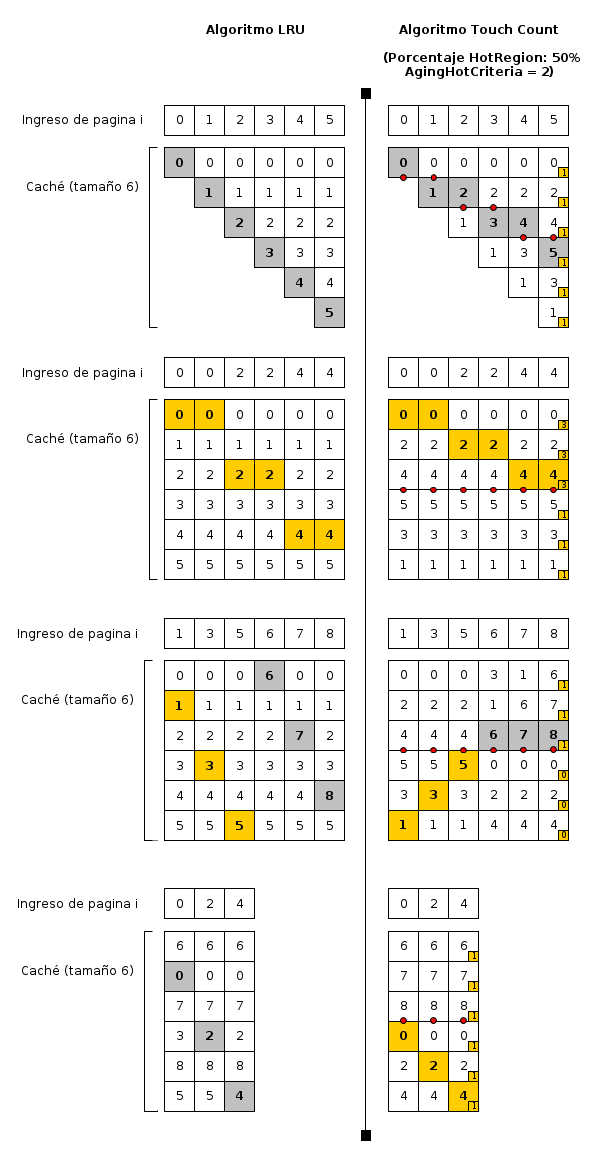
\includegraphics[scale=0.65]{diagramas/LRUvsTouchCountAll.png}\\
	\end{center}

	%\begin{center}
	%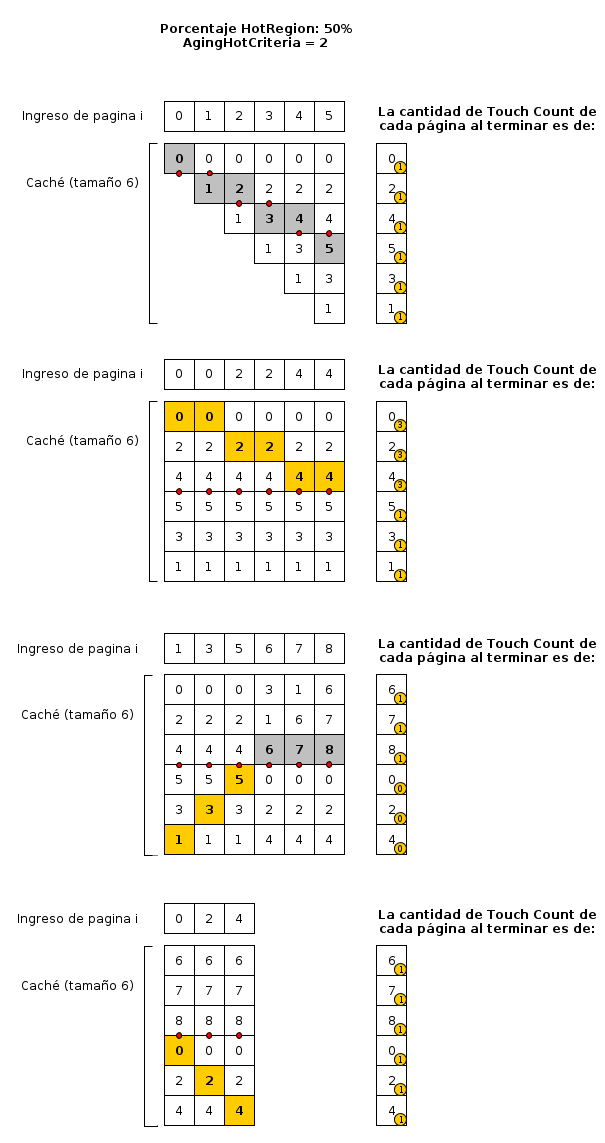
\includegraphics[scale=0.65]{diagramas/LRUvsTouchCount2.png}\\
	%\end{center}

	\subsection{ Mejor caso LRU}
	\subsection{ Mejor caso MRU}
	\subsection{ Mejor caso \textit{Touch Count}}
	\subsection{ Peor caso \textit{Touch Count}}

\end{document}
